\section{configobj::Interpolation\-Loop\-Error Class Reference}
\label{classconfigobj_1_1InterpolationLoopError}\index{configobj::InterpolationLoopError@{configobj::InterpolationLoopError}}
Inheritance diagram for configobj::Interpolation\-Loop\-Error::\begin{figure}[H]
\begin{center}
\leavevmode
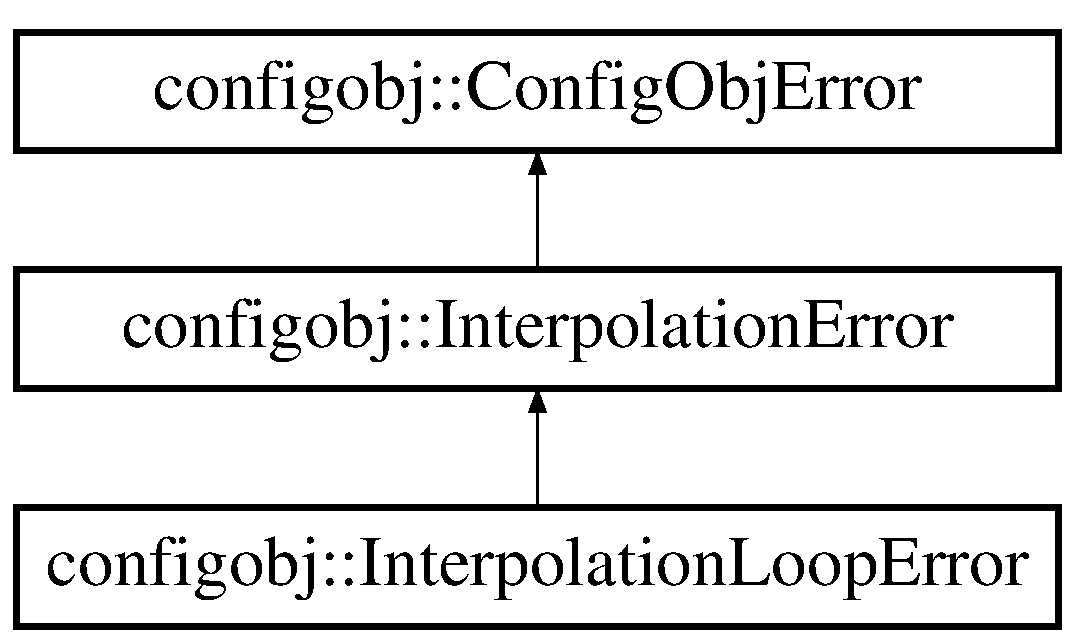
\includegraphics[height=3cm]{classconfigobj_1_1InterpolationLoopError}
\end{center}
\end{figure}
\subsection*{Public Member Functions}
\begin{CompactItemize}
\item 
def \textbf{\_\-\_\-init\_\-\_\-}\label{classconfigobj_1_1InterpolationLoopError_8aad5c776e85e759edae4823a3d5491f}

\end{CompactItemize}


\subsection{Detailed Description}


\footnotesize\begin{verbatim}Maximum interpolation depth exceeded in string interpolation.\end{verbatim}
\normalsize
 



The documentation for this class was generated from the following file:\begin{CompactItemize}
\item 
old/PANICtool-1.0/configobj.py\end{CompactItemize}
